\openepigraph{Memory... is the diary that we all carry about with us.}{---Oscar Wilde}

\section{Lab 4: MiniProject 1 Nairne, Pandeirada, \& Thompson, (2008)}

In the first mini-project, you will read, summarize and discuss the paper by \citeauthor{nairne_adaptive_2008} (2008)\cite{nairne_adaptive_2008}. Then, you will attempt to replicate their results in the lab, by conducting an experiment and analyzing the data.

\subsection{What's in store}
\begin{enumerate}
\item Students read paper and write QALMRI (15-20)
\item Group discussion about paper (15-20)
\item	Students attempt to replicate the major findings in the paper

a.	Break into four-five groups, each group assigned an encoding condition (Survival, Pleasantness, Imagery, Self-reference, Intentional learning)

b.	Each group picks their own 30 words. Can follow same procedure as in paper by choosing 30 words from Overschelde, Rawson, \& Dunlosky (2004) \cite{van_overschelde_category_2004}.

c.	Groups try to run at least 10 participants in their condition, recording proportion of correctly recalled words

d.	Groups enter their collected data into the master spreadsheet, which is given back to groups upon data completion

\item Discussion of how to analyze the data
\item Group attempt to analyze the data using t-tests and one-way ANOVA to determine if the survival framing produced better recall than the other conditions.
\end{enumerate}




\section{Data-analysis tips}\label{lab-4-data-analysis-tips}

In this mini-lab, you will be determining whether different kinds of
manipulations improve your ability to recall lists of words. Each
condition different subjects will read a list a words, and then recall
as many as they can on a sheet of paper. Then, you will measure recall
for each subject by counting the number of correctly recalled words. You
will try to get at least 10 subjects in each condition, the more the
merrier. The empirical question will be whether memory recall is differs
across the conditions. If they do differ, then some of those conditions
help you remember words better, and some conditions may hurt your
ability to remember words. With these kinds of experiments, we can learn
about the factors that influence our memory, as well as how cognitive
processes allow us to encode and retrieve memories.

The new tool you be using here is a one-way ANOVA, which you may
remember from your statistics classes. In particular, we will be
performing an independent samples ANOVA, because we are conducting a
between-subjects experiment, where different subjects contribute data in
each of the conditions. More specifically, we will be conducting an
omni-bus test. The omni-bus test is a catch-all test, that let's us
enter the data from as many conditions as we want, and ask the general
question: are any of the conditions different from one another. This is
different from a t-test, which only let's us make a comparison between
two conditions. In fact, the t-test and ANOVA are related, but this is a
topic that we will leave for now. Except to say, that if you ran a
t-test comparing two groups, or an ANOVA with only two groups, they
would return the same p-values, because they are testing the same
underlying question\ldots{}which is the likelihood the observed occurs
by chance alone.

One drawback about the ANOVA, is that it only tells us if there is some
difference, any difference, among the conditions we are comparing. But,
it does not tell us which specific conditions are different.
Fortunately, after we conduct the ANOVA, we can run follow-up t-tests
comparing any groups we want. We can also conduct more complex
comparisons using linear contrasts, but that is a topic for another day
as well.

We will again use to R to simulate a memory recall experiment with
multiple conditions. Then, we will create fake data, plot the data, then
analyze the data for differences using an ANOVA and follow-up tests.

\subsection{Simulating the data}\label{simulating-the-data}

Consider an experiment with five different memorizing conditions. This
will be a between-subjects experiment with 10 simulated subjects in each
condition. We will have condition A, B, C, D, and E. To simulate data
for each subject we need to make some assumptions. Let's that out of 30
words most people remember about 15 of them, but there is variation, so
some people do better and some people do worse. We can model this by
sampling numbers randomly from a distribution of our choice. For
convenience, we will use the normal distribution, which looks like
bell-curve (should be familiar from statistics class). Let's imagine
that condition A and B help memory more than C and D, and that memory is
worse in condition E. Take a look at the code and output for simulating
this kind of data.

\begin{Shaded}
\begin{Highlighting}[]
\NormalTok{A<-}\KeywordTok{round}\NormalTok{(}\KeywordTok{rnorm}\NormalTok{(}\DecValTok{10}\NormalTok{,}\DecValTok{20}\NormalTok{,}\DecValTok{2}\NormalTok{))}
\NormalTok{B<-}\KeywordTok{round}\NormalTok{(}\KeywordTok{rnorm}\NormalTok{(}\DecValTok{10}\NormalTok{,}\DecValTok{20}\NormalTok{,}\DecValTok{2}\NormalTok{))}
\NormalTok{C<-}\KeywordTok{round}\NormalTok{(}\KeywordTok{rnorm}\NormalTok{(}\DecValTok{10}\NormalTok{,}\DecValTok{15}\NormalTok{,}\DecValTok{2}\NormalTok{))}
\NormalTok{D<-}\KeywordTok{round}\NormalTok{(}\KeywordTok{rnorm}\NormalTok{(}\DecValTok{10}\NormalTok{,}\DecValTok{15}\NormalTok{,}\DecValTok{2}\NormalTok{))}
\NormalTok{E<-}\KeywordTok{round}\NormalTok{(}\KeywordTok{rnorm}\NormalTok{(}\DecValTok{10}\NormalTok{,}\DecValTok{10}\NormalTok{,}\DecValTok{2}\NormalTok{))}
\NormalTok{all_data<-}\KeywordTok{data.frame}\NormalTok{(A,B,C,D,E)}
\KeywordTok{kable}\NormalTok{(all_data,}\DataTypeTok{format=}\StringTok{"latex"}\NormalTok{)}
\end{Highlighting}
\end{Shaded}

\begin{tabular}{r|r|r|r|r}
\hline
A & B & C & D & E\\
\hline
23 & 19 & 17 & 18 & 13\\
\hline
18 & 21 & 17 & 15 & 11\\
\hline
20 & 24 & 16 & 11 & 10\\
\hline
22 & 20 & 15 & 11 & 12\\
\hline
22 & 21 & 12 & 13 & 12\\
\hline
17 & 15 & 15 & 18 & 10\\
\hline
20 & 19 & 14 & 13 & 9\\
\hline
19 & 23 & 17 & 17 & 12\\
\hline
20 & 23 & 13 & 17 & 6\\
\hline
21 & 22 & 19 & 13 & 12\\
\hline
\end{tabular}

We have produced a table with fake data for 10 subjects in each
condition. The numbers all represent the number of correctly recalled
words for each simulated subject. For groups A and B we sample 10
numbers, from a distribution with mean 20, and standard deviation 2.
This is a higher mean than groups C and D (mean = 15). The lowest mean
was for Group E (mean = 10). So, on average, groups A and B should have
higher scores than C and D, which should be higher than E.

Ok, so what happened in our simulated experiment. We can see the numbers
in the table, but it would be nice to summarize them so we can more
easily look at differences. After all, it's hard to make sense of a
bunch of raw data in a table.

One way to summarize the data is to compute the group means for each
condition. This averages over the subjects, and gives us only 5 means to
look at, so it is easier to see the differences. We can ``easily'' do
this in R in a couple different ways. However, R often likes the data in
a particular format, in this case long-data format. So, we will first
convert to that format, and see what it looks like.

\begin{Shaded}
\begin{Highlighting}[]
\NormalTok{long_data<-}\KeywordTok{data.frame}\NormalTok{(}\DataTypeTok{Conditions=}\KeywordTok{rep}\NormalTok{(}\KeywordTok{c}\NormalTok{(}\StringTok{"A"}\NormalTok{,}\StringTok{"B"}\NormalTok{,}\StringTok{"C"}\NormalTok{,}\StringTok{"D"}\NormalTok{,}\StringTok{"E"}\NormalTok{),}\DataTypeTok{each=}\DecValTok{10}\NormalTok{),}
                      \DataTypeTok{Recall=}\KeywordTok{c}\NormalTok{(A,B,C,D,E))}
\KeywordTok{kable}\NormalTok{(long_data[}\DecValTok{1}\NormalTok{:}\DecValTok{25}\NormalTok{,],}\DataTypeTok{format=}\StringTok{"latex"}\NormalTok{)}
\end{Highlighting}
\end{Shaded}

\begin{tabular}{l|r}
\hline
Conditions & Recall\\
\hline
A & 23\\
\hline
A & 18\\
\hline
A & 20\\
\hline
A & 22\\
\hline
A & 22\\
\hline
A & 17\\
\hline
A & 20\\
\hline
A & 19\\
\hline
A & 20\\
\hline
A & 21\\
\hline
B & 19\\
\hline
B & 21\\
\hline
B & 24\\
\hline
B & 20\\
\hline
B & 21\\
\hline
B & 15\\
\hline
B & 19\\
\hline
B & 23\\
\hline
B & 23\\
\hline
B & 22\\
\hline
C & 17\\
\hline
C & 17\\
\hline
C & 16\\
\hline
C & 15\\
\hline
C & 12\\
\hline
\end{tabular}

I've only printed the first 25 lines, but the dataframe contains all of
the data for conditions, C, D, and E as well. You can see why they call
it long format. It's because each data point gets it's own row in the
table.

\subsection{Looking at the means}\label{looking-at-the-means}

Now that the data is in long format we can easily make a table of the
condition means

\begin{Shaded}
\begin{Highlighting}[]
\NormalTok{condition_means<-}\KeywordTok{aggregate}\NormalTok{(Recall~Conditions,long_data,mean)}
\KeywordTok{kable}\NormalTok{(condition_means,}\DataTypeTok{format=}\StringTok{"latex"}\NormalTok{)}
\end{Highlighting}
\end{Shaded}

\begin{tabular}{l|r}
\hline
Conditions & Recall\\
\hline
A & 20.2\\
\hline
B & 20.7\\
\hline
C & 15.5\\
\hline
D & 14.6\\
\hline
E & 10.7\\
\hline
\end{tabular}

We can now see the group means, but we can't see any measure of how
variable the data are in each condition. We might, for example, also
want to compute the standard deviation as well as the mean, and put them
both in the table. We could run the same code from above and substite sd
for mean, which would give us a table of standard deviations. However,
we will use a more advanced function from the plyr package, called
ddply. ddply let's you compute multiple statistics and put them all in a
single table. The syntax is a bit different, but it doesn't take long to
get used to it.

\begin{Shaded}
\begin{Highlighting}[]
\KeywordTok{library}\NormalTok{(plyr)}
\NormalTok{condition_means<-}\KeywordTok{ddply}\NormalTok{(long_data,.(Conditions),summarise,}
                       \DataTypeTok{MeanRecall=}\KeywordTok{mean}\NormalTok{(Recall),}
                       \DataTypeTok{StdDeviation=}\KeywordTok{sd}\NormalTok{(Recall))}
\KeywordTok{kable}\NormalTok{(condition_means,}\DataTypeTok{format=}\StringTok{"latex"}\NormalTok{)}
\end{Highlighting}
\end{Shaded}

\begin{tabular}{l|r|r}
\hline
Conditions & MeanRecall & StdDeviation\\
\hline
A & 20.2 & 1.873796\\
\hline
B & 20.7 & 2.626785\\
\hline
C & 15.5 & 2.121320\\
\hline
D & 14.6 & 2.756810\\
\hline
E & 10.7 & 2.057507\\
\hline
\end{tabular}

\subsection{Plotting the data}\label{plotting-the-data}

It's often very desirable to plot the data in a graph, rather than just
present the means in a table. People find it easier to look at graphs,
because the differences in the data just pop-out much easier than
looking at numbers in a table. R has a fantastic graphing package called
ggplot2. ggplot2 is a whole philosophy for visual design and
data-presentation, and it can be daunting at first. But, it's complexity
makes it very powerful, and when you get the hang of it you can very
quickly make all sorts of beautiful graphs to present data. Here is some
code to make ggplot create a bar graph to plot the means, along with
error bars. In this case the error bars with represent standard errors
of the mean, rather than standard deviations. R does not have a built in
function for the standard error of the mean, so we have to write it
ourselves.

\begin{Shaded}
\begin{Highlighting}[]
\KeywordTok{library}\NormalTok{(ggplot2)}
\NormalTok{sde<-function(x)\{}\KeywordTok{sd}\NormalTok{(x)/}\KeywordTok{length}\NormalTok{(x)\}}
\NormalTok{plot_means<-}\KeywordTok{ddply}\NormalTok{(long_data,.(Conditions),summarise,}
                       \DataTypeTok{MeanRecall=}\KeywordTok{mean}\NormalTok{(Recall),}
                       \DataTypeTok{SE=}\KeywordTok{sde}\NormalTok{(Recall))}

\NormalTok{limits <-}\StringTok{ }\KeywordTok{aes}\NormalTok{(}\DataTypeTok{ymax =} \NormalTok{MeanRecall +}\StringTok{ }\NormalTok{SE, }\DataTypeTok{ymin =} \NormalTok{MeanRecall -}\StringTok{ }\NormalTok{SE)}

\KeywordTok{ggplot}\NormalTok{(plot_means,}\KeywordTok{aes}\NormalTok{(}\DataTypeTok{x=}\NormalTok{Conditions, }\DataTypeTok{y=}\NormalTok{MeanRecall))+}
\StringTok{  }\KeywordTok{geom_bar}\NormalTok{(}\DataTypeTok{position=}\StringTok{"dodge"}\NormalTok{,}\DataTypeTok{stat=}\StringTok{"identity"}\NormalTok{)+}
\StringTok{  }\KeywordTok{geom_errorbar}\NormalTok{(limits, }\DataTypeTok{width=}\NormalTok{.}\DecValTok{1}\NormalTok{)+}
\StringTok{  }\KeywordTok{theme_classic}\NormalTok{(}\DataTypeTok{base_size=}\DecValTok{12}\NormalTok{)+}
\StringTok{  }\KeywordTok{ylab}\NormalTok{(}\StringTok{"Mean Correctly }\CharTok{\textbackslash{}n}\StringTok{ Recalled Words"}\NormalTok{)+}
\StringTok{  }\KeywordTok{xlab}\NormalTok{(}\StringTok{"Condition"}\NormalTok{)}
\end{Highlighting}
\end{Shaded}

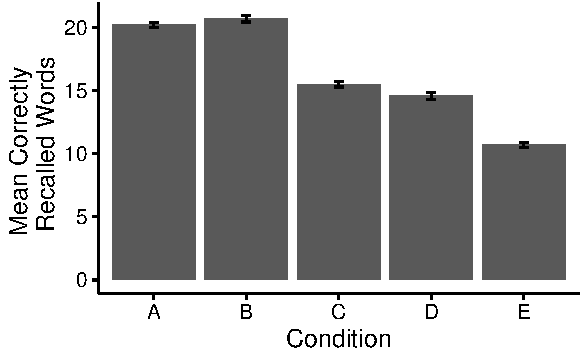
\includegraphics{Lab4_files/figure-latex/unnamed-chunk-5-1}

Now it is easy to the differences between conditions. Just as we had
hoped, Groups A and B appear to have recalled more words than Groups C
and D, which remembered more words than group E.

\subsection{Conducting the ANOVA}\label{conducting-the-anova}

Although the graph and the tabe show some clear differences in the
means, we still want to find out the probability that this kind of
finding occurs by chance alone. We can be confident in the differences
when we know that they do not occur very often by chance alone. The
first step is conduct a one-way ANOVA. This is very easy in R.

\begin{Shaded}
\begin{Highlighting}[]
\NormalTok{aov.out<-}\KeywordTok{aov}\NormalTok{(Recall~Conditions,long_data)}
\end{Highlighting}
\end{Shaded}

We're done! It's only one line of code. However, we need a couple more
to see the results.

\begin{Shaded}
\begin{Highlighting}[]
\NormalTok{aov_summary<-}\KeywordTok{summary}\NormalTok{(aov.out)}
\KeywordTok{kable}\NormalTok{(}\KeywordTok{xtable}\NormalTok{(aov_summary),}\DataTypeTok{format=}\StringTok{"latex"}\NormalTok{)}
\end{Highlighting}
\end{Shaded}

\begin{tabular}{l|r|r|r|r|r}
\hline
  & Df & Sum Sq & Mean Sq & F value & Pr(>F)\\
\hline
Conditions & 4 & 694.52 & 173.630000 & 32.46095 & 0\\
\hline
Residuals & 45 & 240.70 & 5.348889 & NA & NA\\
\hline
\end{tabular}

The ANOVA table gives us a bunch of information. We will go into much
greater detail about the meaning of each number in the table, but also
assume for now that you are somewhat familiar with these ideas because
you have already taken statistics, right?

We are mainly interested in the p-value, which tells how often results
like the ones we found can occur by chance. But, when we report the
results of our ANOVA, we also provide additional information about the
F-value, the degrees of freedom values, and the mean squared error term.
The reason is that if you know these numbers, you can actually
reconstruct all of the other numbers. The results of our ANOVA are
significant. You could report this in a sentence like the following.

The main effect of condition was significant, F(4, 45) = 32.46, MSE =
5.35, p \textless{} .001.

\subsection{Comparisons between
conditions}\label{comparisons-between-conditions}

The p-value from above is much smaller than .05, which shows the
difference between conditions in the data does not occur very often by
chance alone. However, because we conducted an omni-bus test, we only
know that there is some difference between conditions, but we do not
know which specific conditions are different from one another.

So, we have to conduct additional tests between specific conditions.
There are multiple strategies for conducting these tests. For now, we
will simply run t-tests between comparisons of interest.

Remember, our data simulated the pattern that memory recall would be
better for groups A and B, which would be better than groups C and D,
which would better than group E. In other words A=B \textgreater{} C=D
\textgreater{} E.

We can confirm this pattern by conducting tests to see if it holds up.
For example, how would we test the pattern A=B \textgreater{} C=D
\textgreater{} E, all of the following comparisons need to be true,

\begin{itemize}
\item
  A = B
\item
  A \textgreater{} C
\item
  A \textgreater{} D
\item
  B \textgreater{} C
\item
  B \textgreater{} D
\item
  C = D
\end{itemize}

and, all of the conditions should be greater than E

\begin{itemize}
\item
  A \textgreater{} E
\item
  B \textgreater{} E
\item
  C \textgreater{} E
\item
  D \textgreater{} E
\end{itemize}

Let's conduct a few of these tests, and then report the findings.

\begin{Shaded}
\begin{Highlighting}[]
\KeywordTok{library}\NormalTok{(broom)}
\CommentTok{#conduct t-tests}
\NormalTok{ab<-}\KeywordTok{tidy}\NormalTok{(}\KeywordTok{t.test}\NormalTok{(A,B,}\DataTypeTok{var.equal =} \OtherTok{TRUE}\NormalTok{))}
\NormalTok{ac<-}\KeywordTok{tidy}\NormalTok{(}\KeywordTok{t.test}\NormalTok{(A,C,}\DataTypeTok{var.equal =} \OtherTok{TRUE}\NormalTok{))}
\NormalTok{cd<-}\KeywordTok{tidy}\NormalTok{(}\KeywordTok{t.test}\NormalTok{(C,D,}\DataTypeTok{var.equal =} \OtherTok{TRUE}\NormalTok{))}
\NormalTok{de<-}\KeywordTok{tidy}\NormalTok{(}\KeywordTok{t.test}\NormalTok{(D,E,}\DataTypeTok{var.equal =} \OtherTok{TRUE}\NormalTok{))}

\CommentTok{#put the results in a table}
\NormalTok{alltests<-}\KeywordTok{rbind}\NormalTok{(ab,ac,cd,de)}
\NormalTok{alltests<-}\KeywordTok{cbind}\NormalTok{(alltests,}\DataTypeTok{Comparison=}\KeywordTok{c}\NormalTok{(}\StringTok{"AB"}\NormalTok{,}\StringTok{"AC"}\NormalTok{,}\StringTok{"CD"}\NormalTok{,}\StringTok{"DE"}\NormalTok{))}
\NormalTok{finaltable <-}\StringTok{ }\KeywordTok{subset}\NormalTok{(alltests, }\DataTypeTok{select =} \KeywordTok{c}\NormalTok{(Comparison,estimate1,estimate2,statistic,p.value,parameter))}
\KeywordTok{kable}\NormalTok{(finaltable,}\DataTypeTok{format=}\StringTok{"latex"}\NormalTok{)}
\end{Highlighting}
\end{Shaded}

\begin{tabular}{l|r|r|r|r|r}
\hline
Comparison & estimate1 & estimate2 & statistic & p.value & parameter\\
\hline
AB & 20.2 & 20.7 & -0.4900286 & 0.6300329 & 18\\
\hline
AC & 20.2 & 15.5 & 5.2511144 & 0.0000541 & 18\\
\hline
CD & 15.5 & 14.6 & 0.8181818 & 0.4239528 & 18\\
\hline
DE & 14.6 & 10.7 & 3.5851808 & 0.0021158 & 18\\
\hline
\end{tabular}

\subsection{Writing it all up}\label{writing-it-all-up}

The following is an example results section for our hypothetical
experiment. This could serve as a model for your own results section.

The number of correctly recalled words for each subject in each
condition were submitted to a one-way ANOVA, with memorization condition
(A, B, C, D, and E) as the sole between-subjects factor. Mean recall
scores in each condition are displayed in Figure 1.

The main effect of memorization condition was significant, F(4, 45) =
32.46, MSE = 5.35, p \textless{} .001. Figure 1 shows that Groups A and
B had higher recall scores than Groups C and D, which had higher recall
scores than Group E. This pattern was confirmed across four independent
sample t-tests. Group A (M = 20.2) and Group B (M = 20.7) were not
significantly different t(18) = -0.49, p =0.63. Group A recalled
significantly more words than Group C (M = 15.5), t(18) = 5.25, p =0.
Group C and Group D (M = 14.6) were not significantly different t(18) =
0.82, p =0.424. Finally, Group D recalled significantly more words than
Group E (M = 10.7), t(18) = 3.59, p =0.002.









